\documentclass[11pt]{article}

\usepackage{ucs}
\usepackage[utf8x]{inputenc}
\usepackage[T1]{fontenc}
\usepackage{graphicx}
\usepackage{titlesec}

\usepackage[ngerman]{babel}
\usepackage[autostyle=true,german=quotes]{csquotes}

\usepackage[acronym,hyperfirst=false]{glossaries}
\usepackage[colorlinks]{hyperref}

\usepackage{acronym}

\usepackage[colorinlistoftodos,prependcaption]{todonotes}
\usepackage{soul}

% Besseres highlighting von Worten
% https://tex.stackexchange.com/questions/343458/
\makeatletter
\if@todonotes@disabled
\newcommand{\hlnote}[2]{#1}
\else
\newcommand{\hlnote}[2]{\todo{#2}\texthl{#1}}
\fi
\makeatother


\setlength{\parskip}{1.5em}

\titlespacing*{\section} {0pt}{0ex}{0ex}
\titlespacing*{\subsection} {0pt}{0ex}{0ex}
\titlespacing*{\subsubsection} {0pt}{0ex}{0ex}

\title{Abschlussarbeit}
\author{Tom Hilge}

\makeglossaries

\newacronym{JWT}{JWT}{JSON Web Token}
\newacronym{URI}{URI}{Uniform Resource Identifier}
\newacronym{HTTP}{HTTP}{Hypertext Transfer Protocol}
\newacronym{CSS}{CSS}{Cascading Style Sheets}
\newacronym{JSON}{JSON}{JavaScript Object Notation}
\newacronym{MVC}{MVC}{Model View Controller}
\newacronym{HTML}{HTML}{Hypertext Markup Language}
\newacronym{DOM}{DOM}{Document Object Model}
\newacronym{SPA}{SPA}{Single Page Application}
\newacronym{CLI}{CLI}{Command Line Interface}
\newacronym{API}{API}{Application Programming Interface}
\newacronym{RFC}{RFC}{Request for Comments}
\newacronym{MIME}{MIME}{Internet Media Type}
\newacronym{HMAC}{HMAC}{Keyed-Hash Message Authentication Code}
\newacronym{SHA256}{SHA256}{Secure Hash Algorithm 256 Bit}
\newacronym{oAuth2}{oAuth2}{Open Authorization 2.0}

\begin{document}
	
	\section{Einführung}
	\label{sec:introduction}
	Aktuell ist in Blattwerkzeug keine Benutzer-Authentisierung, -Authentifizierung und -Autorisierung implementiert. Dies hat zur Folge, dass  zum jetzigen Zeitpunkt jeder Blattwerkzeug-Nutzer dazu autorisiert ist, jegliche, vom Client erlaubten, Änderungen vorzunehmen. Dies resultiert aus dem bisher einzigen Nutzer in der Datenbank. Das Adminpanel ist beispielsweise für jeden Blattwerkzeug-Nutzer, über die Seiten-Navigation, frei zugänglich. Im Rahmen dieser Thesis soll genau dieses Problem gelöst werden. Nach Behandlung der Thesis soll es möglich sein, sich mit einer standardisierten Registrierung bei Blattwerkzeug anzumelden. Außerdem soll es ebenfalls möglich sein, sich über externe Anbieter anzumelden. Zusätzlich soll je nach Benutzerrolle und Benutzergruppe des angemeldeten Nutzers unterschiedlicher Inhalt dargestellt werden.
	
	\section{Technologien}
	\label{sec:technology}
	Im Verlauf dieser Sektion werden die Technologien und deren Verwendungszweck
	kurz erläutert.

	\subsection{Blattwerkzeug}
	\label{sec:blattwerkzeug}
	
	\begin{figure}
		
\includegraphics[scale=0.4]{images/blattwerkzeug.png}
	\end{figure}
	
	
	Blattwerkzeug ist ein quelloffenes Projekt, dass Informatik-Interessierten das Programmieren von \gls{HTML} Grundgerüsten und SQL Statements per \enquote{drag and drop} näher bringen kann. Dabei versteckt Blattwerkzeug den Syntax nicht vor dem Nutzer, sondern gibt ihm die Möglichkeit diesen gleich mit ein zu sehen. Dennoch ist es dem Nutzer einfach gemacht, mit visuellen Elementen teile der Informatik kennen zu lernen.
	
	Dabei hat es sich Blattwerkzeug vor allem als Aufgabe gemacht an Schulen aufzutreten. Mit Blattwerkzeug wird Lehrern ein Werkzeug in die Hand gelegt, mit dem einfacher und informativer Informatik Unterricht gestaltet werden kann. Somit kann der veraltete und doch sehr Office-lastige Informatik Unterricht komplett erneuert und interessanter gestaltet werden\todo{Zuviel: BlattWerkzeug ist ein Zusatz, keine Ersetzung}.
	
	Zu dem aktuellen Zeitpunkt ist in Blattwerkzeug keine Benutzer Authentisierung, Authentifizierung und Autorisierung implementiert. Dies hat zur Folge.
	
	\subsection{Passwort Hashing}
	\label{sec:password_hashing}
	
	Sobald eine Software mit Nutzerdaten geführt wird, ergibt sich das Problem des speicherns der Passwörter jeweiliger Nutzer.
	Denn sollten die Daten der Nutzer im Klartext in der Datenbank gespeichert werden und ein Angreifer erlangt Zugriff auf die Datenbank, so ist es für ihn ein leichtes weitere Konten der Nutzer zu infiltrieren. Der Grund dafür sind die anwendungsübergreifenden, vom Nutzer größtenteils identischen, Passwörter.
	
	An diesem Punkt kommt das Hashen von Passwörtern zum einsatz. Passwort Hashing soll dem Nutzer Sicherheit gewährleisten und es einem Angreifer nicht möglich machen mit erlangten Daten weitere Konten der Nutzer zu infiltrieren. Dabei wird aus einem Passwort ein Hash generiert, dieser Hash macht es einem unmöglich, das Passwort wiederherzustellen. Jedoch ergibt sich bei gleicher Eingabe, der gleiche Hash. Um ein gehashtes Passwort zu erhalten, muss ein Hashing Algorithmus auf das jeweilige Klartext Passwort angewendet werden.
	
	Mittlerweile gibt es verschiedene Hash-Funktionen, von denen manche als nicht mehr sicher gelten. \hlnote{Bestimmte}{Weasel} Menschen haben es sich zur Aufgabe gemacht sogenannte Rainbowtables~\ref{fig:rainbowtable} zu erstellen, in denen Hashes mit dazugehörigem Klartext Passwort stehen. Dies hat zur Folge, dass falls ein Angreifer die Nutzerdaten erlangt und die Passwörter mit einer solchen Hash-Funktion gehasht wurden. Die Möglichkeit besteht das gehashte Passwort mit einer Rainbowtable abzugleichen und dabei das jeweilige Klartext Passwort zu erhalten. Weshalb MD5~\ref{fig:md5} und SHA zwei der bekanntesten Hash-Funktionen, seit geraumer Zeit nicht mehr zum Passwort hashen verwendet werden.
	
	\begin{figure}[h]
sec:introduction		\includegraphics[width=\textwidth]{images/hash-md5.png}
		\caption{Resultat einer MD5 Hashfunktion auf ein Klartext.}
		\label{fig:md5}
	\end{figure}

	\begin{figure}[h]
		\includegraphics[width=\textwidth]{images/rainbowtable.png}
		\caption{Beispiel einer Rainbowtable.}
		\label{fig:rainbowtable}
	\end{figure}
	
	Aus diesem Grund werden sogenannte Salts~\ref{fig:salted-hash}, zufällig generierte Zeichenketten, an das Passwort angehängt und darauf folgend die Hashfunktion angewandt.

	\begin{figure}[h]
		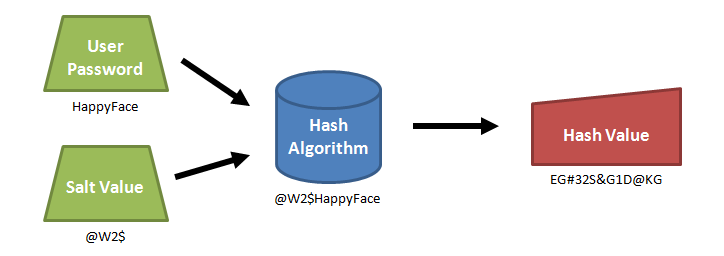
\includegraphics[width=\textwidth]{images/salted_hash.png}
		\caption{Hashfunktion auf Klartext und Salt angewandt.}
		\label{fig:salted-hash}
	\end{figure}
		
	\subsection{Sessions}
	\label{sec: sessions}
	
	Das \gls{HTTP} ist ein zustandsloses Protokoll, dass sich keine Informationen der jeweiligen Aufrufe zwischenspeichert. Dies ist unpraktisch, da so keine Informationen des Nutzers kurzzeitig gespeichert werden können. Ein Verwendungszweck wäre beispielsweise der Warenkorb, da dieser nur temporär vorhanden sein soll. Genau dieses Problem kann mit der Session gelöst werden.
	
	Die Session ist eine serverseitige Daten-Speichermöglichkeit. Dabei wird bei der Anfrage von einem Client an den Server ohne Session-ID eine Session und Session-ID erstellt. Diese Session-ID wird bei der Antwort des Servers mit an den Client ausgeliefert. Ab diesem Punkt wird bei jeder Anfrage vom Client an den Server die Session-ID mit gesendet. Dies kann über einen Cookie oder über die \gls{URI} erfolgen. Aufgrund dessen kann der Server dem Client Daten aus der jeweiligen Session zur Verfügung stellen.
	
	IMAGE
	
	\newpage
	
	\subsection{JSON Web Token}
	\label{sec: jwt}
	\enquote{\gls{JWT} sind auf \gls{JSON} basierende \gls{RFC} 7519 genormte Access-Token.} \gls{RFC} ist eine Sammlung aus Dokumenten in denen das Verhalten der Technologien des Internets beschrieben ist. Einige davon gehören zum Standart und werden somit in den meisten Fällen vorrausgesetzt. In speziellen Fällen möchte beispielsweise ein Unternehmen eigene Protokolle verwenden die nicht zum Standart gehören. 
	
	Diese Tokens werden zur eindeutigen Identifizierung von Nutzern verwendet und können die Session ersetzen. Dabei ist es bei einem \gls{JWT} nicht von nöten die Daten auf dem Server zu speichern. Dies hat zur Folge, dass die Pflege des Speichers an diesem Punkt entfällt. Jedoch haben \gls{JWT} einen großen Nachteil, sobald der Server einen \gls{JWT} ausgestellt hat, ist dieser bis zum Ablauf des Tokens gültig. Das heißt, sollte ein Server die Berechtigung eines Nutzers nach Austellung eines \gls{JWT} ändern, ist diese Änderung erst bei erneutem erstellen eines \gls{JWT} gültig.
	
	Ein \gls{JWT} besteht aus Header, Payload und Signatur. Dabei ist der Header und die Payload jeweils ein \gls{JSON} Objekt.
	
	\subsubsection{Header}
	\label{sec: jwt_header}
	
	\begin{description}
		\leftskip=1em
		\item[typ] Der typ Claim beschreibt den \gls{MIME} des \gls{JWT}, dieser wiederum teilt dem Client oder Server mit um welche Art von Medium an Daten es sich handelt. Der Stanart-Wert dieses Claims beläuft sich auf \enquote{JWT}, übersetzt \enquote{application/jwt}.
		\item[alg] Der alg Claim beschreibt die Verschlüsselungsmethode. Ein Beispiel ist \gls{HMAC} mit \gls{SHA256}, HS256 abgekürzt.
	\end{description}
	
	\begin{figure}[h]
		\includegraphics[width=\textwidth]{images/jwt-header.png}
		\caption{Beispiel eines \gls{JWT} Headers }
		\label{fig:jwt-header}
	\end{figure}
	
	\subsubsection{Payload}
	\label{sec: jwt-payload}
	
	Die Payload beinhalteten Schlüssel-Wert Paare werden Claims genannt. Dabei handelt es sich um ein JSON Objekt, bei dem bestimmte Schlüssel des Objektes bereits reserviert sind. Diese nennen sich registrierte Claims. Außerdem gibt es öffentliche und private Claims. Hierbei wird zwischen öffentlichen und privaten differenziert.
		
	\noindent
	\textbf{Beispiel registierter Claims}
	
	\begin{description}
		\leftskip=1em
		\item[iss]
		Der iss Claim steht für den Austeller des Tokens, beispielsweise eine Domain.
		\item[exp] Der exp Claim kennzeichnet den \gls{JWT} mit einem Ablaufdatum.
	\end{description}
	
	\todo[inline]{Mehr konkrete Beispiele, weniger Breite}

	\noindent
	\textbf{Öffentliche Claims}

	Öffentliche Claims sind zusätzlich zum Standart nutzbar und ihre Namen sollten Semantisch dem dazugehörigen Wert entsprechen. Außerdem sollten die Namen der Claims Netzwerkübergreifend verständlich sein.~\ref{fig:public-claim}

	\noindent
	\textbf{Private Claims}

	Private Claims werden nur innerhalb eines Netzwerkes verwendet. Aus diesem Grund gibt es keine implizite Beschrenkung in der Namensgebung.~\ref{fig:private-claim}  
	
	\begin{figure}[h]
		\centering
		\includegraphics[width=\textwidth]{images/public-claim.png}
		\caption{Öffentlicher Claim eines \gls{JWT} }
		\label{fig:public-claim}
	\end{figure}
	
	\begin{figure}[h]
		\centering
		\includegraphics[width=\textwidth]{images/private-claim.png}
		\caption{Privater Claim eines \gls{JWT} }
		\label{fig:private-claim}
	\end{figure}
	
	\subsubsection{Signatur}
	\label{sec: jwt_signature}
	
	Um die Signatur zu erhalten muss die Payload und der Header Base64 kodiert werden. Außerdem müssen diese beiden kodierten Zeichenfolgen mit einem Punkt als Trennzeichen verknüpft werden. Darauf folgend wird eine Hashfunktion auf das jeweilige Ergebnis mit zusätzlich sicherer Zeichenfolge als Parameter angewandt. Da diese sichere Zeichenfolge, auch Private Key genannt, nur auf dem Server hinterlegt ist, ist es dem Client zwar möglich den \gls{JWT} zu verändern, ihn jedoch mit korrekter Signatur zu versehen nicht.
	
	\subsubsection{Zusammengesetzes Token}
	\label{sec: jwt_result}
	Schlussendlich ergibt sich der \gls{JWT} aus kodierten Header, kodierten Payload und der Signatur. Dabei steht der Header am Anfang Abbildung \ref{fig:jwt-encoded} Rot gekennzeichnet. Darauf folgend mit einem Punkt getrennt die Payload und zum Schluss die Signatur, ebenfalls mit einem Punkt getrennt.
	
	\begin{figure}[h]
		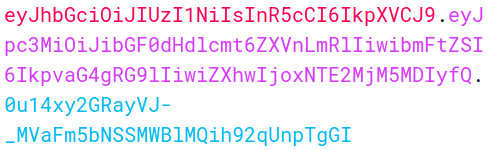
\includegraphics[width=\textwidth]{images/jwt-encoded.png}
		\caption{Beispiel eines codierten \gls{JWT} }
		\label{fig:jwt-encoded}
	\end{figure}
	
	\subsection{Ruby on Rails}
	\label{sec: rails}
	Ruby on Rails ein quelloffenes Webframework für die Programmiersprache Ruby. Das Webframework nutzt das \gls{MVC} Muster und stellt bereits ein sehr umfangreiches \gls{CLI} zur Verfügung. Mittels des generate Werkzeugs kann beispielsweise Model, View und Controller erstellt werden. Jeder dieser Komponenten wird automatisch in die erstellte Rails Anwendung eingebunden. Außerdem stellt Rails eine umfangreiche Test-Architektur und einen Service zum versenden von Mails. Dabei kann der Inhalt der E-Mail im Textformat oder als \gls{HTML} versendet werden. Einer der wesentlichen Vorteile von Ruby on Rails ist jedoch die Datenbankanbindung. Hierbei bietet Rails einen Nachhaltigen und Rücksichtsvollen Umgang mit der Datenbank, beispielsweise Migrationen. Migrationen erlauben die Datenbank, ohne explizite SQL-Statements, zu verändern. Außerdem erleichtern Migrationen die Implementierung einer Datenbankstruktur auf einem anderen System.
	
	\todo[inline]{Nochmal in den eigenen Quelltext schauen: Welche Aspekte sind wirklich relevant?}
	
	\subsubsection{Routen}
	\label{sec: routen}
	Die Routen in Rails verweisen auf einen Controller und auf eine Funktion innerhalb des Controllers. Dabei wird die Route meistens mit der Anfragemethode eingeleitet, beispielsweise \enquote{get}. Routen können in sogennante \enquote{scopes}~\ref{fig:routes-scope} unterteilt werden. Somit ist es nicht von nöten bei einer Verschachtelten \gls{URI} redundant zu werden.~\ref{fig:routes-redundant}
	
	\begin{figure}
		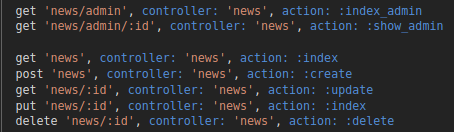
\includegraphics[width=\textwidth]{images/routes-redundant.png}
		\caption{Beispiel einiger redundanter Routen }
		\label{fig:routes-redundant}
	\end{figure}
	
	\begin{figure}
		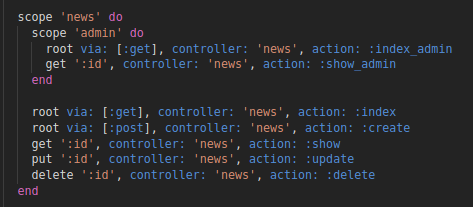
\includegraphics[width=\textwidth]{images/routes-news.png}
		\caption{Beispiel einiger Routen mit scope }
		\label{fig:routes-scope}
	\end{figure}
	
	\subsubsection{Controller}
	\label{sec: rails_controller}
	Der Controller dient hierbei zur Kapselung von bestimmten Prozessen. Jede Route verweist in irgendeiner Weise auf eine Controller Funktion. In der der jeweiligen Controller Funktion wird dann meistens mit einem Model interagiert. Es wird beispielsweise eine Benutzerberechtigung abgefragt und individuell auf die Berechtigung reagiert. Um auf die jeweilige Berechtigung zu reagieren gibt es mehrere Möglichkeiten. Eine der Möglichkeiten wäre, direkt ein View Template auf dem Server zu rendern und an den Client auszuliefern. Eine andere Möglichkeit wäre ein \gls{JSON} Objekt zurück zu geben und darauf mit dem Client zu agieren.
	
	\subsubsection{Model}
	\label{sec: rails_model}
	Das Model in Rails stellt jeweils eine Datenbanktabelle dar. Die Attribute des Models sind jeweilige Spalten der Datenbanktabelle. Jeweilige Datenbankeinträge die über das Model erstellt werden, können mittels Validatoren auf ihre Gültigkeit geprüft werden. Diese Validatoren werden innerhalb des Models festgelegt und auf ein Attribut des Models zugewiesen. Rails bietet dabei bereits verfügbare Validatoren, beispielsweise \enquote{presence: true} \hlnote{IMAGE-REF}{Bild Referenz}. Dieser Validator sorgt für das Vorhanden sein eines Wertes ungleich \textit{nil}. Jedes Model kann zusätzliche Funktionen beinhalten, die direkt auf den jeweiligen Datenbankeintrag angewandt werden kann. Außerdem bietet Rails die Möglichkeit die Beziehungen zwischen Datenbanktabellen direkt in den Modellen festzulegen.
	
	\subsubsection{View}
	\label{sec: rails_view}
	Die View stellt in Rails die Möglichkeit \gls{HTML} Template auf dem Server zu rendern. Dabei kann beim rendern das \gls{HTML} Template dynamisch verändert werden. Da diese Komponente während dieser Thesis keine Rolle gespielt hat, wird diese nicht weiter erläutert.
	
	\subsection{Zusammenfassung}
	\label{sec: rails_resuemee}
	Schlussendlich wird über die Route auf den jeweiligen Controller zugegriffen. Dieser fragt in den meisten Fällen nach einem bestimmten Eintrag eines Models. Darauf folgend wird mit dem Ergebnis der Anfrage interagiert. Es werden Veränderungen oder abfragen bestimmter Daten getätigt. Danach wird ein Ergebnis dem Client ausgeliefert.
	
	\subsection{Angular}
	\label{sec: angular}
	Angular ist ein TypeScript basiertes Front-End Webframework, dass in vielen fällen für \gls{SPA} verwendet wird. \gls{SPA}s laden ihren Inhalt lediglich in ein einziges \gls{HTML} Dokument. Der Inhalt dieses \gls{HTML} Dokumentes wird dynamisch, von beispielsweise einem Framework wie Angular, verändert. Der wesentliche Vorteil von Angular sind die klaren Entwurfsmuster. Jede Komponente in Angular hat im wesentlichen die gleiche Struktur. Dies hat zur Folge, dass Angular eine sehr gute Codekonsistenz bietet.
	
	
	\subsubsection{Component}
	\label{sec: ang-component}
	Komponenten in Angular bieten die Möglichkeit \gls{HTML}, \gls{CSS} und TypeScript zu kapseln. Das bedeutet, dass jede Komponente unabhängig von einer anderen Komponente arbeiten kann.
	
	\subsubsection{Services}
	\label{sec: ang-service}
	Zur kommunikation mit einem Server und/oder zum Datenaustausch zwischen unterschiedlichen Komponenten wird meistens ein Service verwendet. Jedoch bei einem Datenaustausch zwichen Eltern- und Kindkomponente ist es einfacher dies mittels der Kindkomponente durchzuführem. Services werden beim laden der Module instaziert und dem Konstruktor der Komponente als instanziertes Objekt übergeben.
	
	\subsubsection{Module}
	\label{sec: ang-modul}
	Zusätzlich bietet Angular außerdem die Möglichkeit eigene Module zu erstellen in denen dann beispielsweise Services und Komponenten zusätzlich abgekapselt werden können. Ein Vorteil von Angular gegenüber anderen JavaScript Frameworks, sind die bereits von Angular mitgelieferten Module, beispielsweise das Routing- oder das HTTP-Modul. Das Routing-Modul wird für jegliche Navigation auf der Anwendung genutzt. Das \gls{HTTP}-Modul hingegen bietet die Möglichkeit mittels jeglicher Anfragemethoden, mit dem Server zu kommunizieren.
	
	\subsection{oAuth2}
	\label{sec: oauth2}
	\gls{oAuth2} ist ein offenes \gls{RFC} 6749 Protokoll welches verwendet wird um eine Authentifizierung einer Anwendung mittels Drittanbieter zu ermöglichen. Hierbei wird der Nutzer zuerst auf die jeweilige Seite des Drittanbieters weitergeleitet. Dort muss der Nutzer sich authentifizieren und den Zugriff auf die Daten seines Kontos bestätigen. Nachdem der Zugriff auf die Daten bestätigt wurde, erhält die jeweilige Anwendung von dem Drittanbieter einen Autorisierungs-Token. Dieser Autorisierungs-Token wird darauf folgend von der Anwendung genutzt um einen Zugriffs-Token von dem Drittanbieter zu erhalten. Dieser ermöglicht schlussendlich den Zugriff auf die spezifischen Nutzerdaten des Drittanbieters.~\ref{fig:oauth2}
	
	In Blattwerkzeug wird genau dieser umfangreiche Vorgang von Omniauth übernommen. Aus diesem Grund wird oAuth2 in dieser Thesis nicht weiter erläutert.
	
	\begin{figure}[h]
		\includegraphics[width=\textwidth]{images/oauth2.png}
		\caption{oAuth2 verfahren}
		\label{fig:oauth2}
	\end{figure}

	\subsection{Omniauth}
	\label{sec: omniauth}
	Omniauth ist eine quelloffene Library für Ruby on Rails und ermöglicht einem, eine Anmeldung mittels unterschiedlicher Anbieter über \gls{oAuth2}. Bei der Anmeldung mittels oAuth2 werden bereits viele Funktionen von Omniauth selber übernommen. Sobald der Nutzer sich bei dem jeweiligen Anbieter angemeldet hat, wird die Antwort des jeweiligen Anbieters automatisch über die von Omniauth festgelegte Route verarbeitet. Jedoch muss vorher das spezifische Gem des Anbieters für Omniauth installiert werden.
	
	Omniauth selber verfügt nur über die Developer Strategie, diese ermöglicht eine Anmeldung ohne spezifische Überprüfung der angegebenen Daten. Das hat zur Folge, dass diese Art von Anmeldung auf keinen Fall im Produktiv System vorhanden sein darf.
	
	Den Vorteil den Omniauth bietet ist die Kapselung zwischen den spezifischen Providern und der Hauptfunktionalität von Omniauth. Dies hat zur Folge, dass der Server nur explizit mit den installierten Providern kommunizieren kann. Außerdem bietet Omniauth eine lange Liste an zu installierenden Providern.~\ref{fig:provider-list}
	
	\begin{figure}[h]
		\includegraphics[width=\textwidth]{images/provider-list.png}
		\caption{Beispiele einiger zu installierender Provider}
		\label{fig:provider-list}
	\end{figure}

	\subsection{Pundit}
	\label{sec: pundit}
	Pundit ist eine Ruby on Rails Library die ein Designpattern zur Autorisierung bietet. Bei diesem Pattern wird zu einem jeweiligen Controller eine Policy angelegt. Eine Policy ist hierbei nur eine Klasse. Dabei setzt sich der Name der Policy, aus dem Namen des Models und dem Schlüsselwort Policy als Suffix zusammen. Dem Konstruktor der Policy wird ein Nutzer und das jeweilige Objekt übergeben, welches auf den Zugriff geprüft werden soll. Innerhalb der Policy werden die jeweiligen Controllerfunktionsköpfe in denen eine Autorisierung stattfinden soll mit einem \enquote{?} als Suffix ergänzt und definiert. Diese Funktionen müssen zwingend einen Boolean als Rückgabewert haben um eine gültige Auswirkung als Policy zu haben. Sobald die aufgerufene Funktion der Policy fehlschlägt wird eine Exception geworfen. Diese Exception kann an jeweiliger Position beispielsweise im Controller abgefangen und verarbeitet werden. 
	
	Da es sich bei Policies um Klassen handelt, können diese auch instanziert und jeweilige Funktionen dynamisch abgerufen werden. Dies hat zur Folge, dass explizit nach einer bestimmten Policy-Funktion gefragt werden kann, selbst wenn der Funktionsname nicht dem der aufgerufenen Policy-Funktion entspricht.
	
	\subsection{Rolify}
	\label{sec: rolify}
	Rolify ist eine Ruby on Rails Library zur Verwaltung von Rollen. Hierbei liefert Rolify bereits zwei Datenbanktabellen im Design der polymorphen Assoziation. 
	
	
	\section{Problemanalyse}
	\label{sec: analyze}
	
	\section{Implementierung}
	\label{sec: implementation}
	
	\subsubsection{Omniauth Identity\todo{$\rightarrow$Implementierung}}
	\label{sec: omniauth_identity}
	Omniauth Identity ist eine Library zur Erweiterung von Omniauth. Mit Omniauth Identity ist intern ein Anbieter gegeben mit dem es möglich ist, sich zusätzlich mit einem Passwort zu registrieren und anzumelden. Eben so wie die Developer Strategy, bietet auch diese Library die Möglichkeit ein vorgefertigtes Formular für Anmeldung und Registrierung zu erstellen. Jedoch ist es bei dieser Library optional und eine auschließliche Kommunikation über ein API ist möglich. 
	
\end{document}
%%% Local Variables:
%%% mode: latex
%%% TeX-engine: xetex
%%% TeX-master: t
%%% End:
